\chapter{Background \& Related Work}
In this chapter, relevant background knowledge and related previously published work is discussed.

\section{Magnetic Resonance Imaging}
\subsection{Fundamentals of MRI}
%% RAD 229 Lect-01 A
MRI uses the ability of certrain nuclei to absorb and emit energy in the radio frequency spectrum to generate images of organisms.
This ability is called Nuclear Magnetic Resonance and depends on charge, spin, and mass, which are the intrinsic properties of particles. \\
\textbf{Nuclear Magnetic Resonance-active Nuclei} are those atoms with  with an odd number of protons and/or neurtons\autocite{nishimura, halliday}.
They have a spin angular momentum defined as
\[ S = \hbar I, \]
where $I$ is the spin operator and $\hbar$ is Planck's constant normalized by $2\pi$.
The odd number of protons/neutrons also induces a magnetic dipole moment
\[ \mu = \gamma S. \]
$\gamma \ [\text{MHz} / \text{T}]$ is called the gyromagnetic ratio and is unique to each nuclear magnetic resonance-active nuclei.
It is the ratio of the magnetic dipole moment $\mu$ to the spin of a particle $S$.
The gyromagnetic ratio governs the frequency of precession and is meassured empirically. \\
Specifically, ${}^1$H has a spin of $0.5$, a high natural abundance of $0.998$ and is therefore used primarily for clinical and medical MRI.
its gyromagnetic ratio is $\gamma = 42.57$ MHz$/$T.\\
When placing such nucleie into a magnetic field, the spins have a tendency to align with its direction, leading to a net or bulk magnetization per unit volume (or voxel) $v$,
\[ M = \sum_{v \in V} \mu_v. \]
Additionally, due to spin and mass, the nucleus exhibits an angular momentum, i.e. it precesses e.g. in a gravitational field.
The dynamics of this angular momentum  or pecession can be described by
\[ \frac{d \mu}{d t} = \mu \times \gamma B, \]
when considering a single nucleus and for a summing over a unit volume
\[ \frac{d M}{d t} = M \times \gamma B. \]
The combination of magnetic and angular momentum causes the nucleus to precess in a magnetic field as well with a specific frequency --- called the Larmor frequency:
\[ \omega = \gamma B, \]
where $B \ [T]$ is the strength of a magnetic field and $\gamma$ is the gyromagnetic ratio.

A scanner MR scanner consists of a primary electromagnetic coil, that is surrounded by a cryostat and thermal insulation, an excitation coil, spatial localization coils, and a receiver coil, as shown in \ref{scanner-teardown}.
The excitation and the receiving coil are merged into one RF coil here. \\
\fig{img/mri-scanner_teardown.png}{scanner-teardown}{MRI scanner with a part cut-away such that the main components are visible.}{0.5}

This \textbf{primary electromagnet} provides the main magnetic field $B_0$ to polarize the NMR-active nuclei with field strengths up to $14.2 T$, but usually about $1.5 T$ to $3 T$ in medical applications.
This is several orders of magnitude larger than the earth magnetic field which is approximately $0.5$ Gauss
To provide such high fields, super-conductivity needs to be reached, thus the coil is cooled using liquid helium.
The $B_0$ field is spatially uniform and temporally stable in an ideal scanner, such that the same polarization is applied to all atoms.
In practice this field is not perfectly homogeneous, such that magnetic field probes are used to measure the field and shim cards are used to correct these inhomogenieties.
This is called passive shimming.
Alternatively, active shimming coils can be used to smooth the inhomogenieties.
It is oriented along the ``long'' part of the scanner, so if a human lies in the scanner, the poles are oriented towards the head and the feet of the subject.
We call this axis the $z$-axis. \\

%% RAD 229 Lect 01 B
Additionally, an \textbf{excitation system} is necessary to generate exciting magnetic pulses $B_1(t)$ to cause nutation of the nuclei of interest as well as to refocussing, spoiling, inversion and saturation.
The $B_1(t)$ field is a radio frequency field with the excitation frequency defined by the $B_0$ field strength, the Larmor frequency of the excitation target nuclei and are both short in duration and amplitude.
For example with $B_0 = 3$T we get
\[ 42.58 \frac{\text{MHz}}{\text{T}} \cdot 3 \text{T} = 127.74 \text{MHz}. \]
Typical pulse durations are on the intervall $[0.1, 10]$ ms and amplitude about $< 25 \mu \text{T}$.
The shape of the excitation pulse is governed by an envelope function in terms of amplitude trajectory.
\fig{img/nutation.png}{nutation}{A visualization of rotation $r$ (in out case we call it spin) in green, precession p in blue --- at the Larmor frequency --- and nutation n in red.}{0.2}
The excitation pulses are perpendicular to the $B_0$ field, which is important to enable the excitation pulses to tip the spin system in the presence of the strong polarizing field.
While the $B_0$ field causes polarization, thus alignment and precession, the $B_1(t)$ pulses cause a ``tipping'' or nutation of the precession --- shown in \ref{nutation}, generating transverse magnetization such that it is detectable using Faraday's law of induction.
An example of an excitation pulse is
\[ B_1(t) = B_1(t)^e (t) \left(\cos\left(\omega_{RF} t + \theta \right) i - \sin\left(\omega_{RF} t + \theta \right) j \right), \]
with $B_1(t)^e (t)$ a pulse envelope function, e.g. \texttt{sinc} or \texttt{rect} functions, $\omega_{RF}$ the excitation carrier frequency which should match the Larmor frequency of the spin system, and $\hat{i}', \ \hat{j}'$ the polarization directions.
Additionally a RF pulse has a filp angle $\alpha$ which is the angle between the $z$-axis and the $B1$ pulse (called inclination in spherical coordinates) and a phase $\theta$ which is the angle in the $xy$ plane, starting at the $x$-axis (azimuth in spherical coordinates).
The excitation system is commonly implemented using a birdcage coil as it's highly efficient in terms of energy, excitation and  heating mitigation.
The $B_1(t)$ field is supposed to be highly uniform, especially radially while decaying slightly axially. \\

A \textbf{receiving coil(s)} reads out the response of the excited tissue.
This can be the same RF coil that is used for excitation.
As the precessing magnetization causes induction in the receiving coil(s), the flux in the receiving coil changes causing an electromotive force
\[ \epsilon = - \frac{\partial \Phi}{\partial t}. \]
The picked up signal is further split up, multiplied by $\cos{\omega_0 t}$ and $\sin{\omega_0 t}$ respectively and low-pass filtered to get the in-phase signal $I(t)$ and the quadrature signal $Q(t)$.
The These signals are then quantized, yielding $I(t)$ as the real and $Q(t)$ as the imaginary part of the signal.

The excitation forces the magnetization off from its equilibrium state and thus induces relaxation back to the equilibrium again after excitation.
This relaxation can be separated into two components: longitudinal and transverse relaxation.

The longitudinal component can be described as a return to the equilibrium state of the magnetization on the $z$-axis
\[ \frac{d M_z}{d t} = - \frac{M_z - M_e}{T_1}, \]
where $M_e$ is the equilibrium nuclear magnetization, which is proportional to the applied magnetic field $B_0$~\autocite{nishimura}.
The solution to this equation is
\[  M_z = M_e + (M_z - M_e) \exp{-t / T_1}. \]
$T_1$ is the time constant of the longitudinal component also called longitudinal relaxation time constant or spin-lattice time constant.
It is proportional to the applied field strength and thus lengthens when $B_0$ is increased in strength.
Practically, it is the time that it takes for $M_z$ to return to $63 \%$ of it's thermal eqilibrium state $M_e$~\autocite{relaxation, lauterbur}.
   \begin{figure}[h]
      \begin{center}
         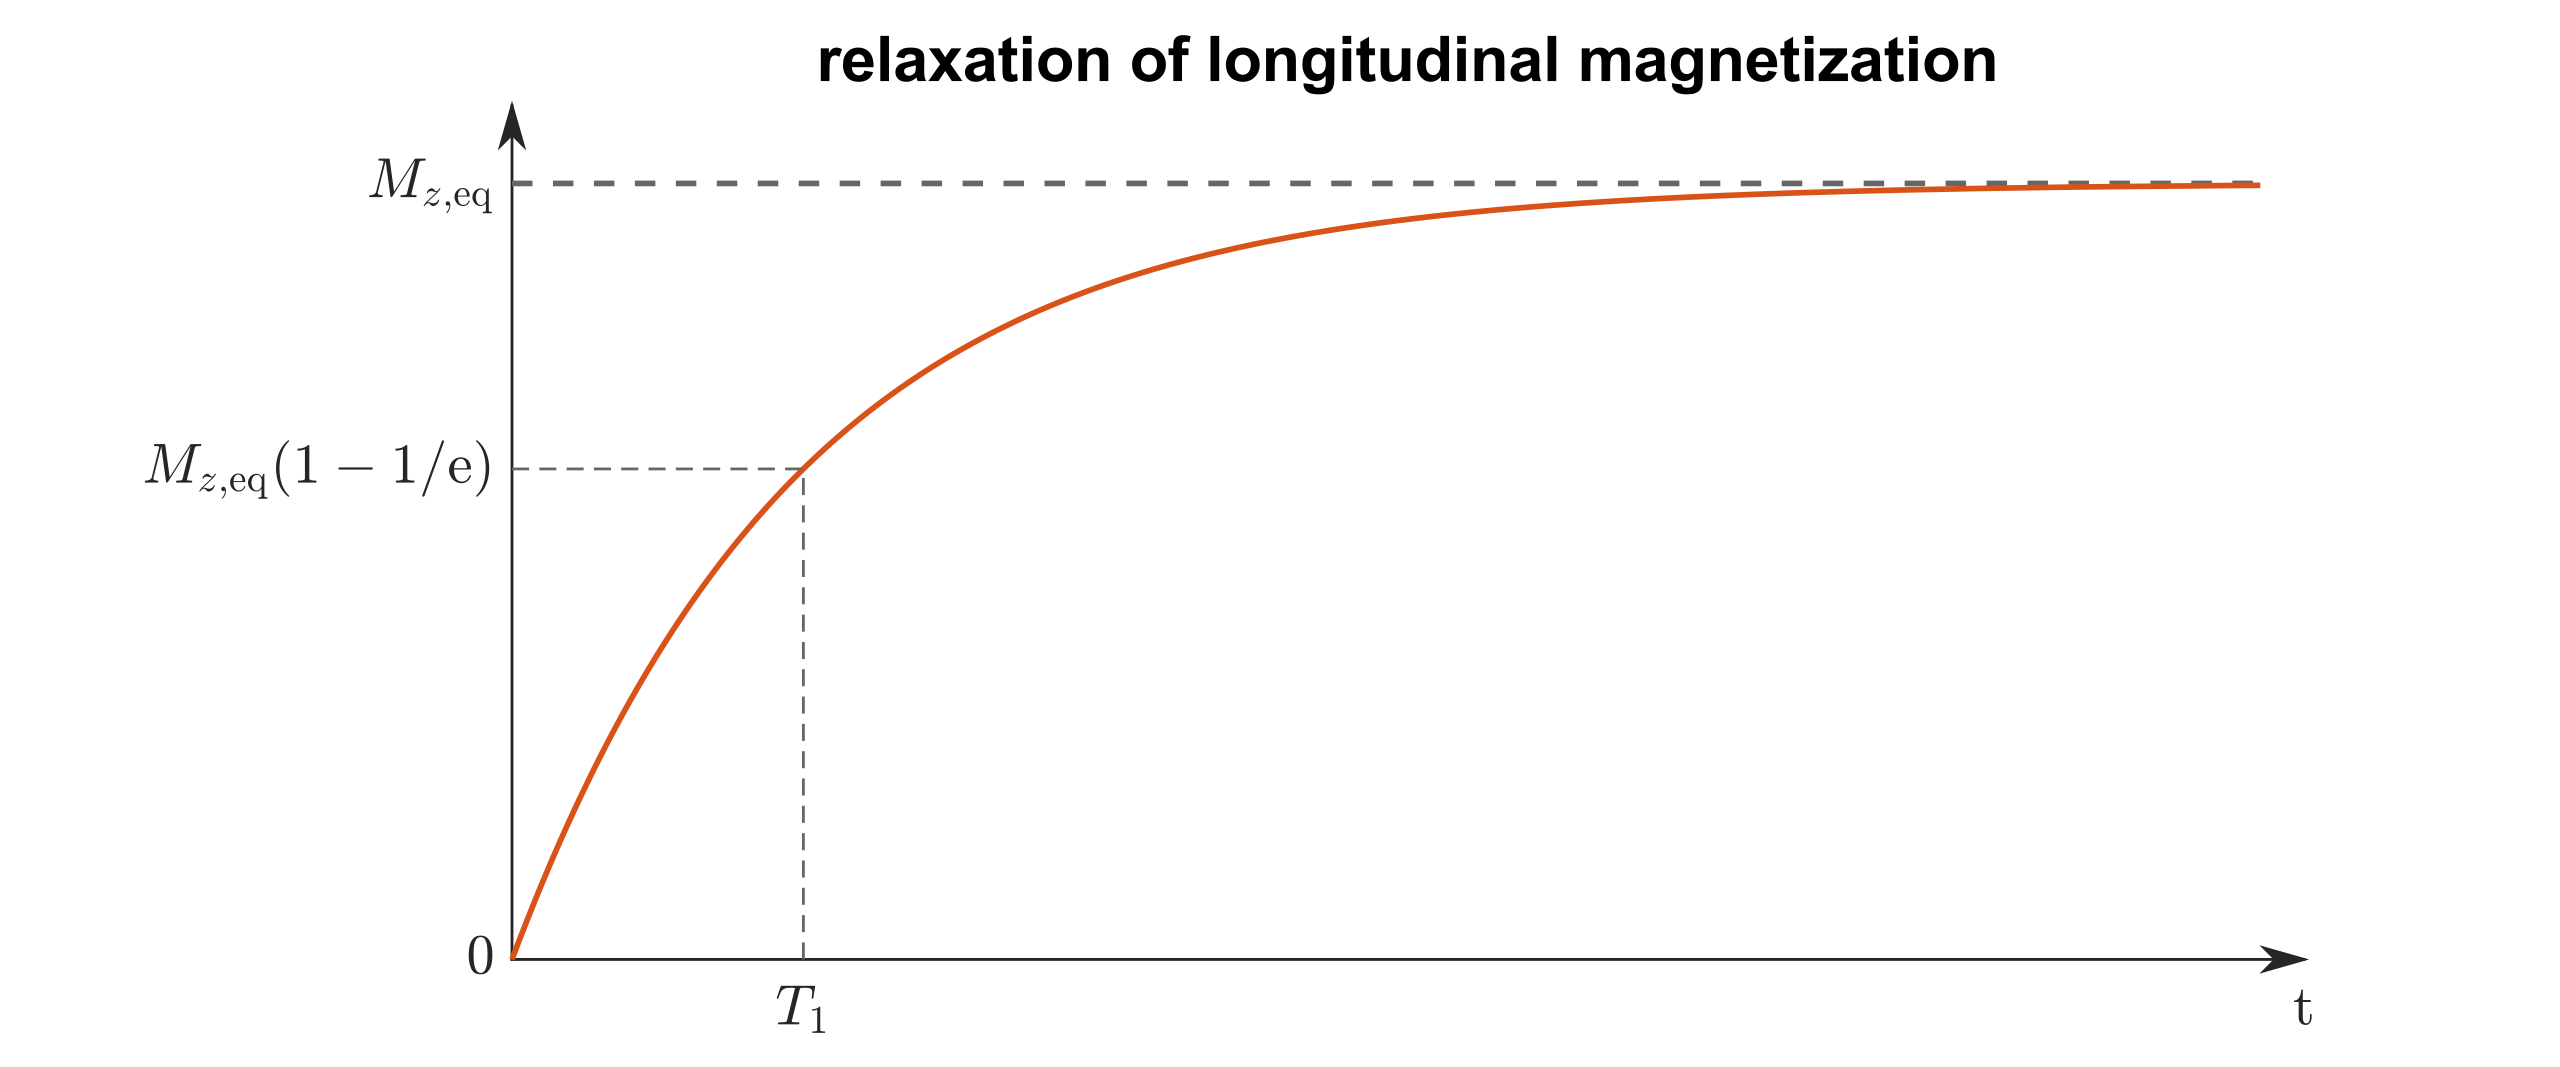
\includegraphics[keepaspectratio, width=0.45\textwidth]{img/t1.png}
         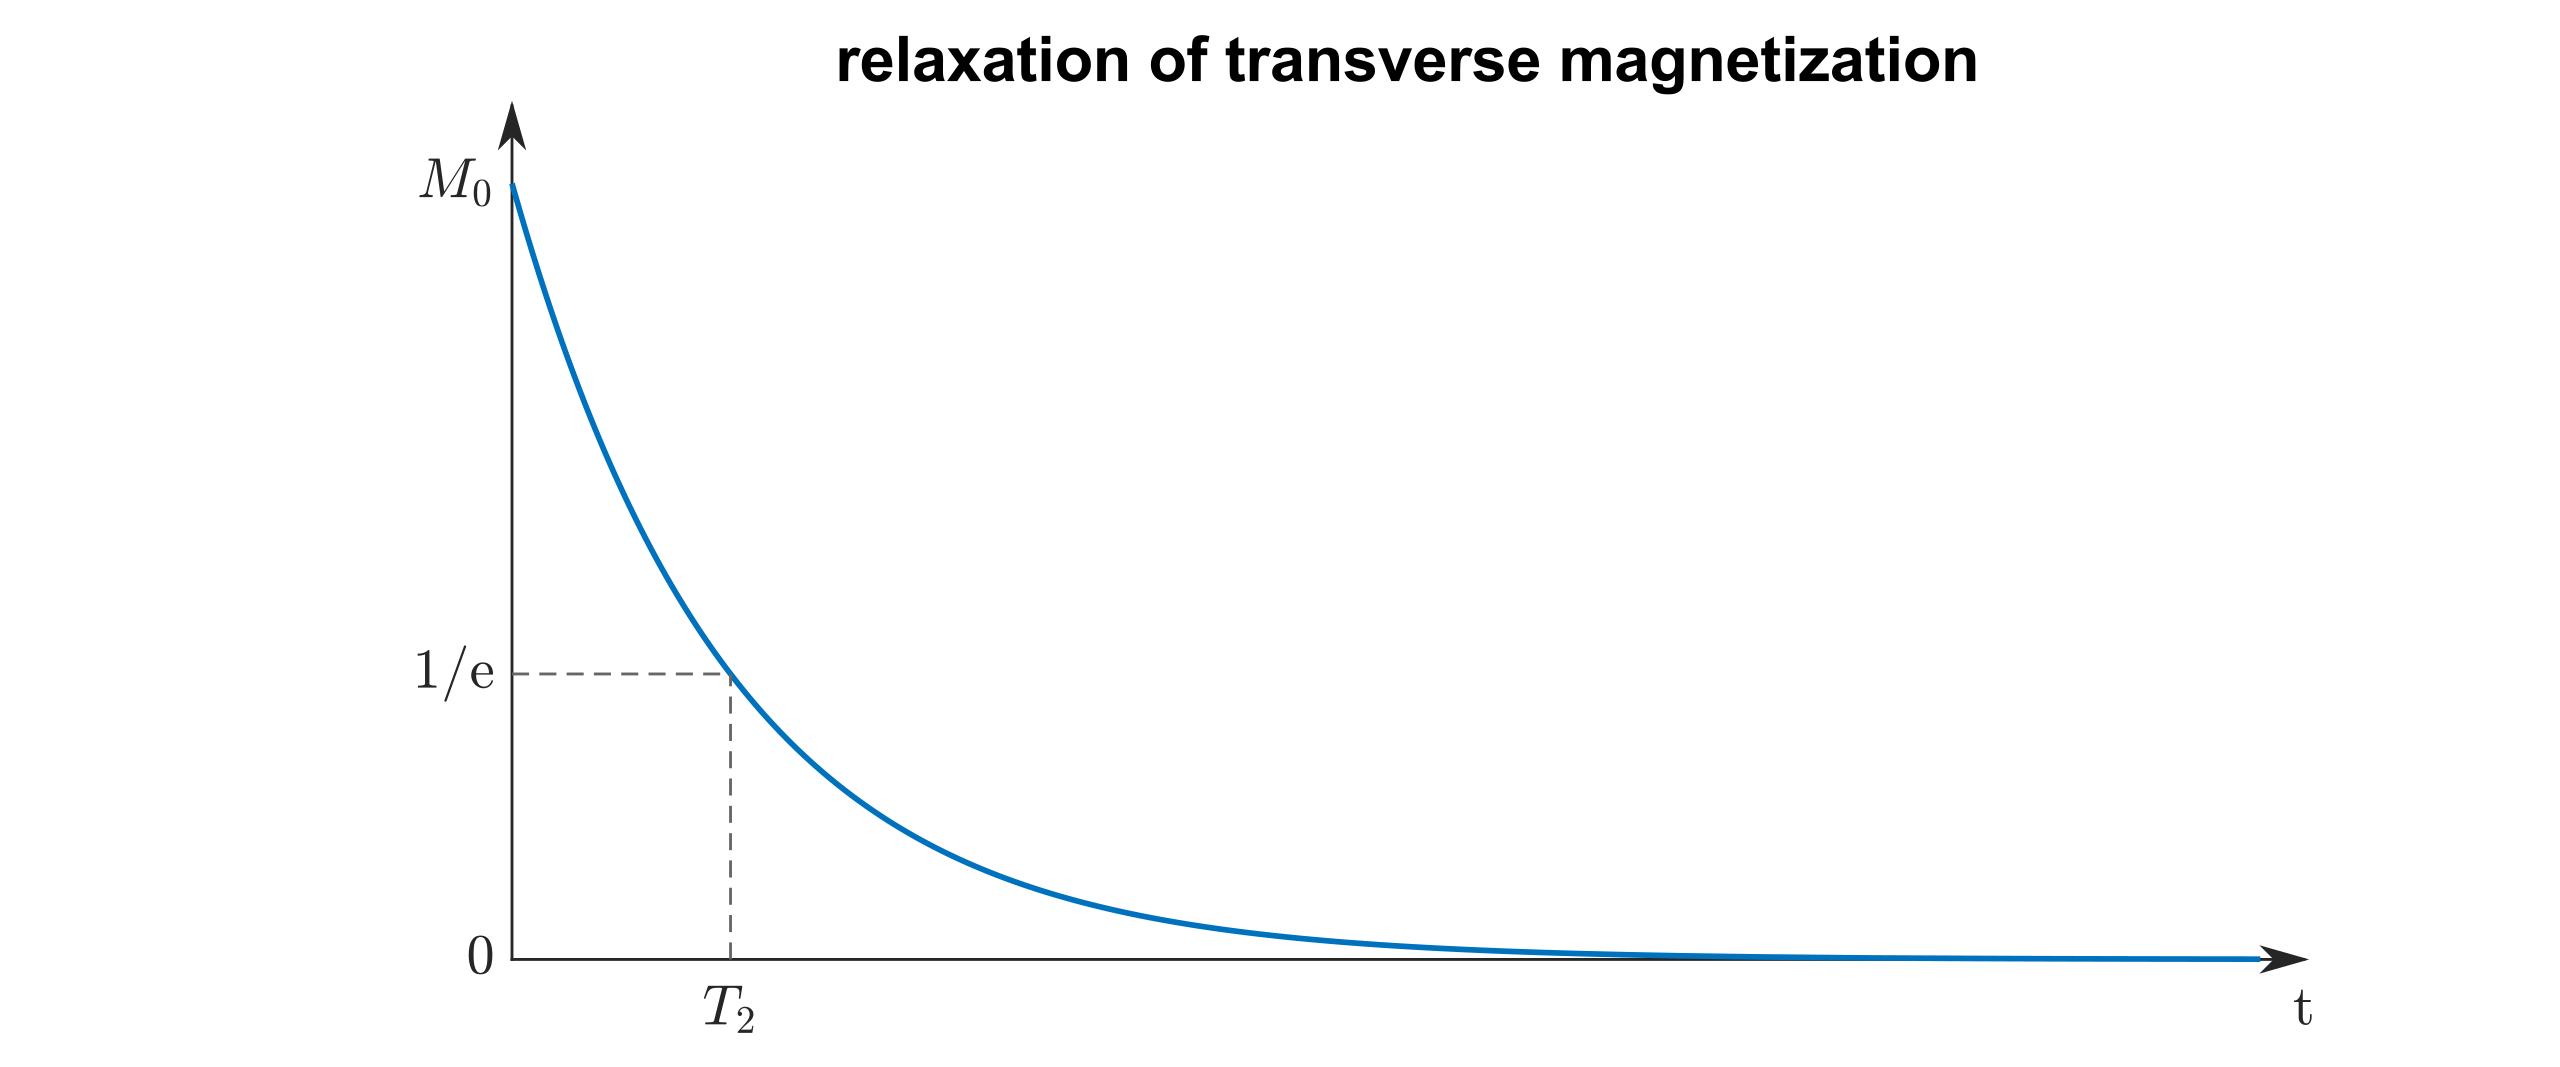
\includegraphics[keepaspectratio, width=0.45\textwidth]{img/t2.png}
      \end{center}
      \caption{
         \textbf{Left:} $T_1$ relaxation curve shows the return to the equilibrium state.
         \textbf{Right:} $T_2$ relaxation curve visualizes the transveral magnetization decay to zero.
      }
      \label{relaxations}
   \end{figure}

The transversal component can be formulated as a decay process
\[ \frac{d M_{xy}}{d t} = - \frac{M_{xy}}{T_2}. \]
Accordingly, $T_2$ is the time constant of the transverse relaxation component, also called spin-spin relaxation time constant.
It is mostly independent from the $B_0$ field strength and $T_2 \leq T_1$.
$T_2$ is more rapid, the less mobile the spins are, i.e. $T_2$ is larger in water than in solids.
Practically, in one $T_2$, $M_{xy}$ loses $63 \%$ of it's magnetization right after excitation.
Typical values for $T_1$ and $T_2$ for common tissue types are shown in table \ref{t1t2-vals}.

\begin{table}[h]
 \begin{tabular}{}
  ×
 \end{tabular}
 \caption{}
 \label{t1t2-vals}
\end{table}



\fig{img/mri_scannercoils.png}{gradient coils}{A conceptual visualization of the gradient coils of an MRI scanner.}{0.4}

%% RAD 229 Lect 02 A
A \textbf{Gradient system} are used to select regions of interest from the full organism and to iterate over different regions. \\



In order to describe the bSSFP sequence later on, the notions of \textbf{the lab and the rotating frame} will be introduced now.
The laboratory frame is the frame of reference from the view in which the room or the scanner is anchored.
The coordinate system is defined based on the $B_0$ field, where the $z$-axis is in the direction of the $B_0$ field, i.e. from the feet of the subject in the scanner to its head.
The $x$-axis is parallel to the floor, while the $y$-axis is parallel to the walls.
Put differently, $y$ corresponds to the height, $x$ to the width and $z$ to the depth of the room.
In this frame, we can observe rotation/spin, precession and rotation.
In contrast, the rotating frame, the rotational/spinning and the precessional behavior is factored out, such that only the nutational information is preserved.
This can be achieved with a transformation of the $xy$-plane, while the $z$-axis stays the same as in the lab frame.
Intuitively, the $xy$ plane in the rotational frame is rotating at frequency $\omega$ relative to the $xy$-axis of the lab frame.

The equation of motion for a system of spins in the lab frame can be described by the Bloch equation, which consists of the precession \& nutation, the transversal and the longitudinal relaxation terms:
\[ \frac{dM}{dt} = M \times \gamma B - \frac{M_x i + M_y j}{T_2} - \frac{(M_z - M_e) k }{T_1}. \]
$B$ aggregates the static $B_0$ field, the excitation $B_1(t)$ field and the gradient $G(t)$ fields.

Let $M_{R} = \left( M_{x'}, M_{y'}, M_z \right)^T$, $B_R = \left( B_{x'}, B_{y'}, B_z \right)$, $R_z$ the rotation matrix around the $z$-axis, $M = R_z(\omega t) M_R$ and $B = R_z(\omega t) B_R$.
When defining the tranverse magnetization as complex $M_R(t) = M_{x'}(t) + M_{y'}(t)$ for the rotating frame and $M(t) = M_x(t) + i M_y(t)$ we can relate the lab and the rotating frame via
\[ M(t) = M_R(t) \exp{-i \omega t} \]
and with $\omega$ the Larmor frequency, $M_{x'}$ and $M_{y`}$ become constants without excitation pulses.
With this we can reformulate the Bloch equation in the rotating frame
\[ \frac{dM}{dt} = M_R \times \gamma B_{\text{eff}} - \frac{M_{x'} i + M_{y'} j}{T_2} - \frac{(M_z - M_e) k }{T_1}, \]
where \[ B_{\text{eff}} = \frac{\omega_R}{\gamma} + B_R \] and $\omega_R = \left( 0, 0, - \omega \right)$.

% Maybe example without relaxation with the typical B1 pulse RAD 229


Finally, Computers control the different coils, store the meassurements and reconstruct images from the meassured magnetizations.
\fig{img/mri-block-diagram.png}{mri-block-diag}{Block diagram of the components in an MRI scanner system}{0.6}

\textbf{Excitation Sequences} \\

%% RAD 229 Lect 09 --- bSSFP
\subsection{balanced Steady-State Free Precession Imaging}

In depth description of sequence, profile, banding

\subsection{Diffusion-weighted Imaging}

\section{Deep Learning}
\subsection{Fundamentals of Neuronal Networks}

\subsection{Architecture \& Training}
UNet, challenges, impact of transformers, ...

\subsection{Image-to-Image Synthesis}

\subsection{Deep Learning in Medical Imaging}



\chapter{Methods}\label{\positionnumber} 
\section{The Dove Dataset}
Some stats on size 
\subsection{Participants \& Study Design}
briefly describe participants, task, scanning times (of the day)

\subsection{Recorded Sequences}
cf gais doc.
Details on acquisitions

\section{Data Processing}
requirements
\subsection{bSSFP}

\subsection{DWI}
TODO ask svenja what was done

\subsection{Augmentation}


\section{Machine Learning-based DWI Tensor estimation from bSSFP data}
MONAI, torchio, pytorch lightning. 

\subsection{Architecture}
UNet + some extra layers to fit output dim.

\subsection{Training}
Pre-training, transfer \& fine-tuning \\

Sparse data, small batch sizes. => Augmentation not enough => Pre training
\paragraph{AutoEncoder PreTraining}
As auto encoder. train autoenc for bssfp only 

\paragraph{ExtraHead Transfer and Fine tuning}
freeze autoenc, add head. transfer then unfreeze all and fine tune
Unet + extra head
